\subsection{Cloud Rendering:}
\label{sec:cr}
There are a number of different processes to use when rendering clouds such as volume rendering.
Due to the nature of clouds when light passes through them it becomes scattered.
The majority of the models looked at the use two different techniques to accomplish this effect: single scattering and multiple scattering.
These models may render clouds using these scattering techniques directly or may use scattering inside other rendering processes such as photon mapping.
A number of these models also use billboards or imposters when rendering the clouds as this saves on computation.
This section will look at volume rendering, single scattering, multiple scattering, and photon mapping.

\subsubsection{Volume Rendering:}
\label{sec:vr}

Volume rendering is the process of converting a 3D set of data and rendering to the screen.
There are two types of volume rendering ray-casting, and slice-based.
This section will look at the first type of volume rendering.
This type of ray casting is done by drawing a ray from the eye position through the 3D object and then calculating the colour of the object by blending the data found whilst iterating through the ray.
Figure \ref{fig:ray_casting2} shows an example of rays being caste from the camera position through the 3D volume.

\begin{figure}[ht!]
	\centering
	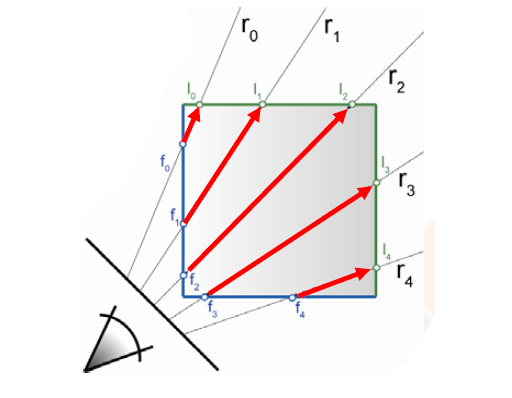
\includegraphics[width=90mm]{images/ray_thumb.PNG}
	\caption{\cite{KHayward09} - Volume Ray Casting}
	\label{fig:ray_casting2}
\end{figure}
\subsubsection{Single Scattering:}
\citet*{MHarris01} describe single scattering as a model that simulates scattering in a single direction that is usually the direction leading to the point of view.
There are debates whether or not this type of rendering is detailed enough for rendering clouds.
\citet{Miyazaki01} states the main topic of his model is the cloud shapes so using single scattering is enough to check the shape of the cloud.
\citet{CBohren87} describes single scattering as insufficient when describing common observations. 
\subsubsection{Multiple scattering:}
\label{sec:multiple}
“Multiple scattering models are more physically accurate, but must account for scattering in all directions … and therefore are much more complicated and expensive to evaluate” \citep{MHarris01}.
\citet{HarrisEtAl03} uses a version of multiple scattering which is called multiple forward scattering, this differs from the original by instead of calculating scattering in all directions it calculates scattering in the forward direction only.
This means the algorithm is less computationally heavy. \citet*{Fedkiw01} describe the multiple scattering of light as necessary for objects made from water vapour, which clouds are.

\subsubsection{Photon Mapping:}
“Photon mapping is a variation of pure Monte Carlo ray tracing in which photons (particles of radiant energy) are traced through a scene” (\citet{Jensen96}, cited in \citet{MHarris03}).
\citet{MHarris03} describes the process of photon mapping as storing position, incoming direction, and radiance of each photon landing on a nonspecular surface that has been traced from the light source.
\citet*{Fedkiw01} use photon mapping when rendering smoke and describe the process as a two pass algorithm, one where a volume photon map is built and the second as a rendering pass using a forward ray marching algorithm.